\chapter{Semi-supervised image segmentation using CNNs in a Bayesian framework}
\section{Training CNN from scribbles}
The use of Variational image processing parametrized with cost learned from RF provides a segmentation mask with good accuracy. The RF was trained with features described in WEKA toolset. These features may not work well for certain medical images and thus, use of CNN proves beneficial as it learns different feature maps according to the task. The initial layers learn basic image features while the final layers get trained for filters to compute problem specific results. In addition to this, the choice of $\lambda$ is always a problem in using VIP. As we showed in section 3.2.2, different parts of images need different values of $\lambda$ to produce best segmentation mask. Ranftl \cite{ranftl:2014} uses CNN with VIP and modifies the loss function accordingly and learns optimal values of $\lambda$ along with CNN parameters. The paper describes a method of combining CNN(5 layers) with a final variational/inference layer. The inference layer has activation function in form of Total variation. Similarly, Taylor et al. \cite{taylor:2016} implemented CNN as a scalable ADMM approach. They split the objective function into subproblems (as we did using ASB) and trained CNN without gradients. These papers attempt to couple CNN with VIP to gain from both approaches. \par

This motivated us to replace RF with CNN to parametrize cost function. In literature, we can find multiple approaches to train CNN using scribbles. Gonda et al.\cite{Gonda:2016} uses an interactive approach to train deep neural networks for segmentation of neuronal structures using scribbles. Lai et al. \cite{Lai:2015} uses patch-based 3D image segmentation. They make use of patches around pixels annotated to train the neural network. A similar approach has been used by Havaei et al.\cite{Havaei:2015} for brain tumor segmentation using deep neural networks. These ideas take each pixel as a sample and CNN is trained as a classifier to classify each pixel. The disadvantage is that we remove one major property of CNN to adapt its final layers according to full image for segmentation task and also, it needs sufficient data to train CNN. Therefore, we tried to train OSVOS network (explained in Section 2) from scribbles using \textbf{cross entropy scribble loss}. The simple trick we used was to replace computation of cross-entropy loss function for the complete image by computing loss for only annotated scribbles. The \textbf{cross entropy scribble loss} can be computed at each pixel, $x$ with probability $p$, as defined below:

\begin{align*}
\funop{l_{scribble}}(x) =
\begin{cases}
  -z(x)\,log(p(x)) - (1 - z(x))\,log(1 - p(x)), & \text{if}\ x \in \text{Scribbles}  \\
  0, & \text{else}
\end{cases}
\end{align*}

We succeeded in training our network with scribble loss and results can be seen in figure 3.11. We compared the results obtained for both RF and CNN using the same amount of pixels annotated. It can be observed that RF looks to perform better for a lower amount of scribbles, while CNN reaches f-measure of a maximum of 0.86 for higher annotation budget.
The mask generated using CNN from scribbles shows uncertainity for pixels at boundaries. Thus, we used Variational image processing over mask obtained from CNN. The boost with VIP can be observed in figure 3.12.
\begin{figure}[h!] \label{fig:cnnvip}
 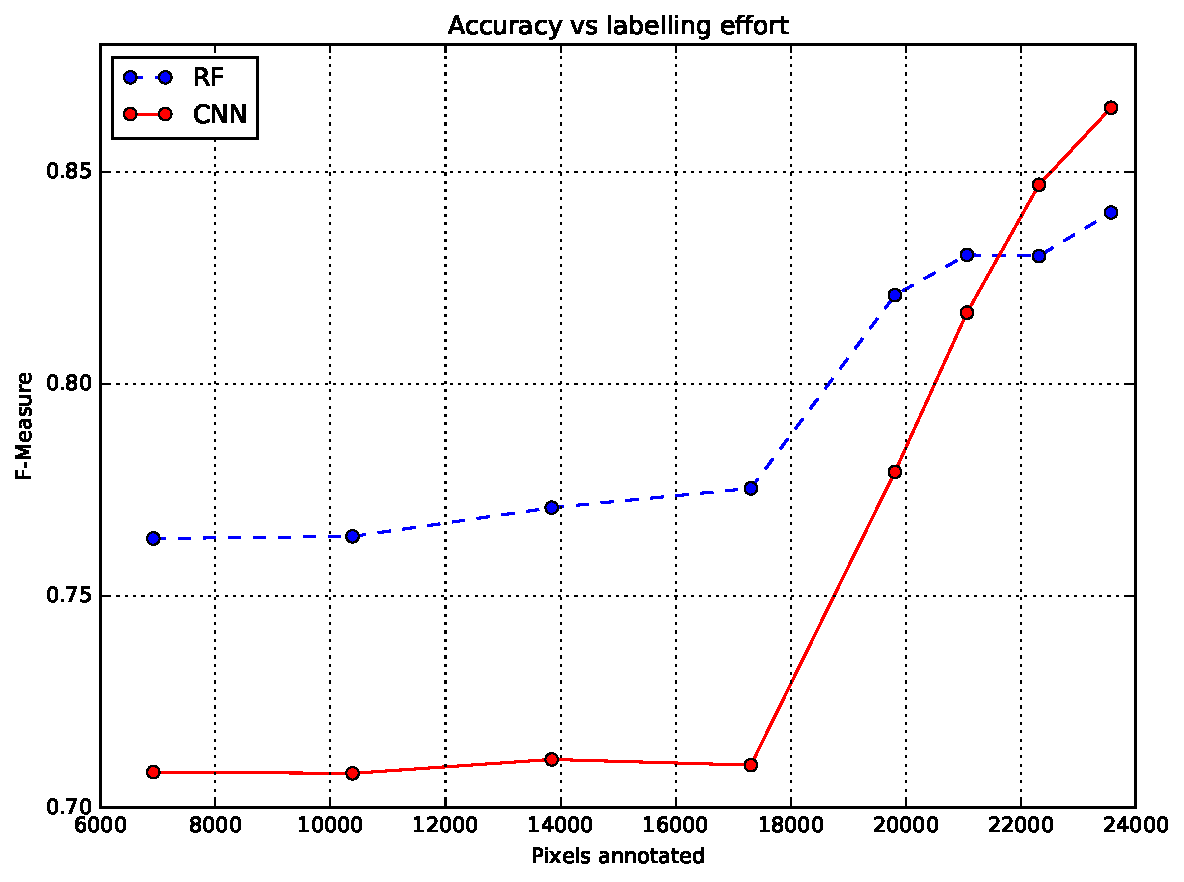
\includegraphics[width=1.0\linewidth]{figures/cnn_vs_rf.pdf} 
\caption{F-measure for increasing annotation budget for comparing CNN vs RF}
\end{figure}

\begin{figure}[h!] \label{fig:cnnvip}
 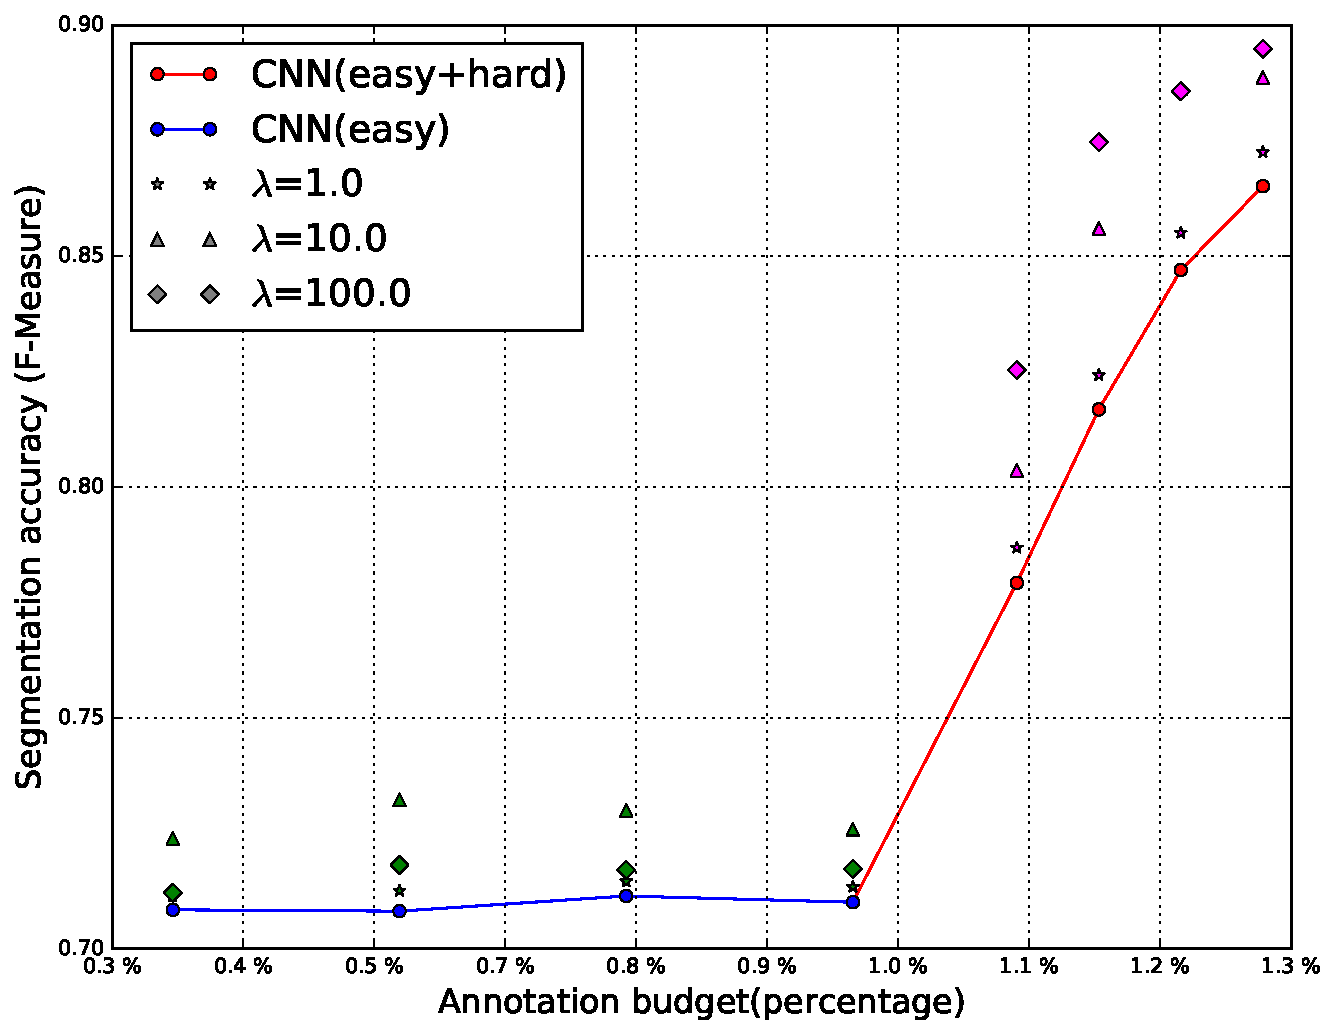
\includegraphics[width=0.8\linewidth]{figures/cnn_vip.pdf}
 \caption{(a) CNN with VIP (different $\lambda$)\, (b) CNN vs RF with VIP}
\end{figure}


\begin{figure}[h!] \label{fig:cnnvip}
 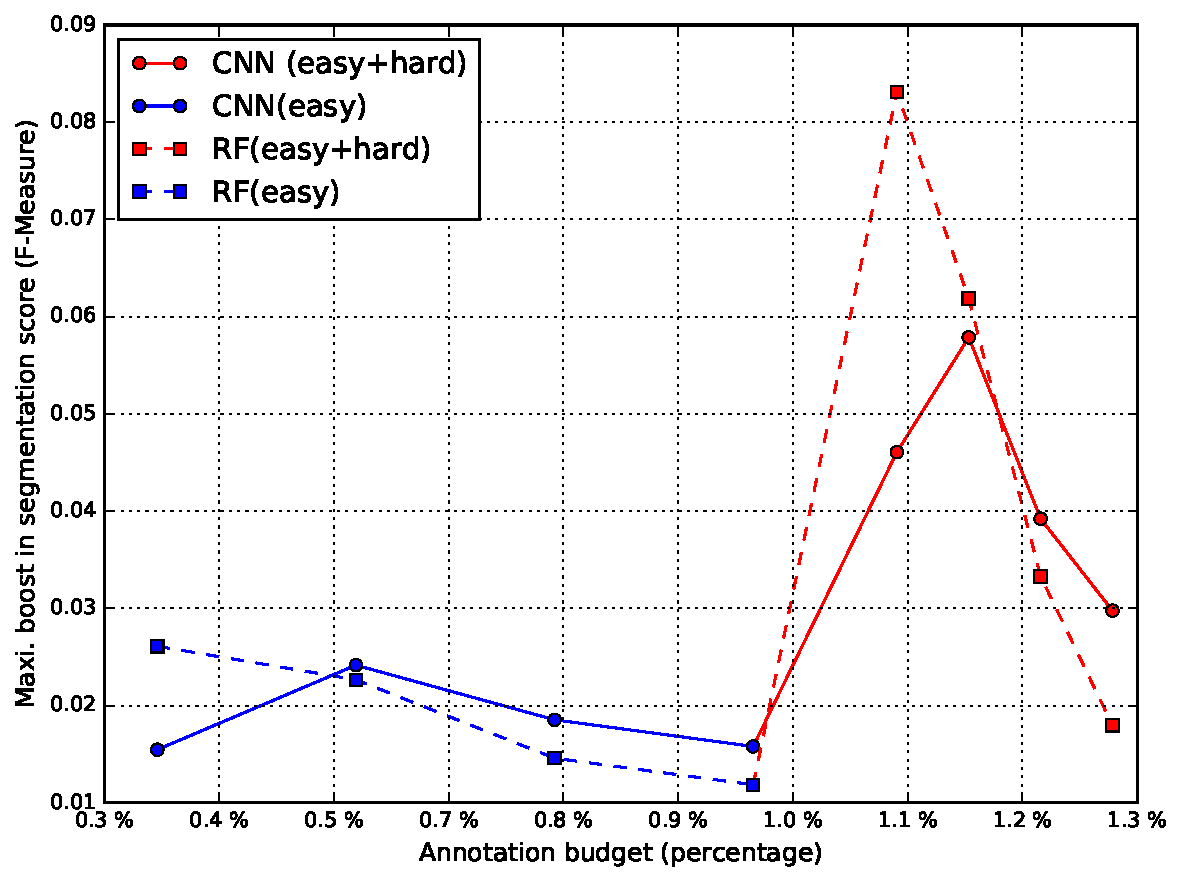
\includegraphics[width=0.8\linewidth]{figures/cnn_vip_boost.pdf}
\caption{(a) CNN with VIP (different $\lambda$)\, (b) CNN vs RF with VIP}
\end{figure}


\begin{figure}[h!] \label{fig:cnnvip}
 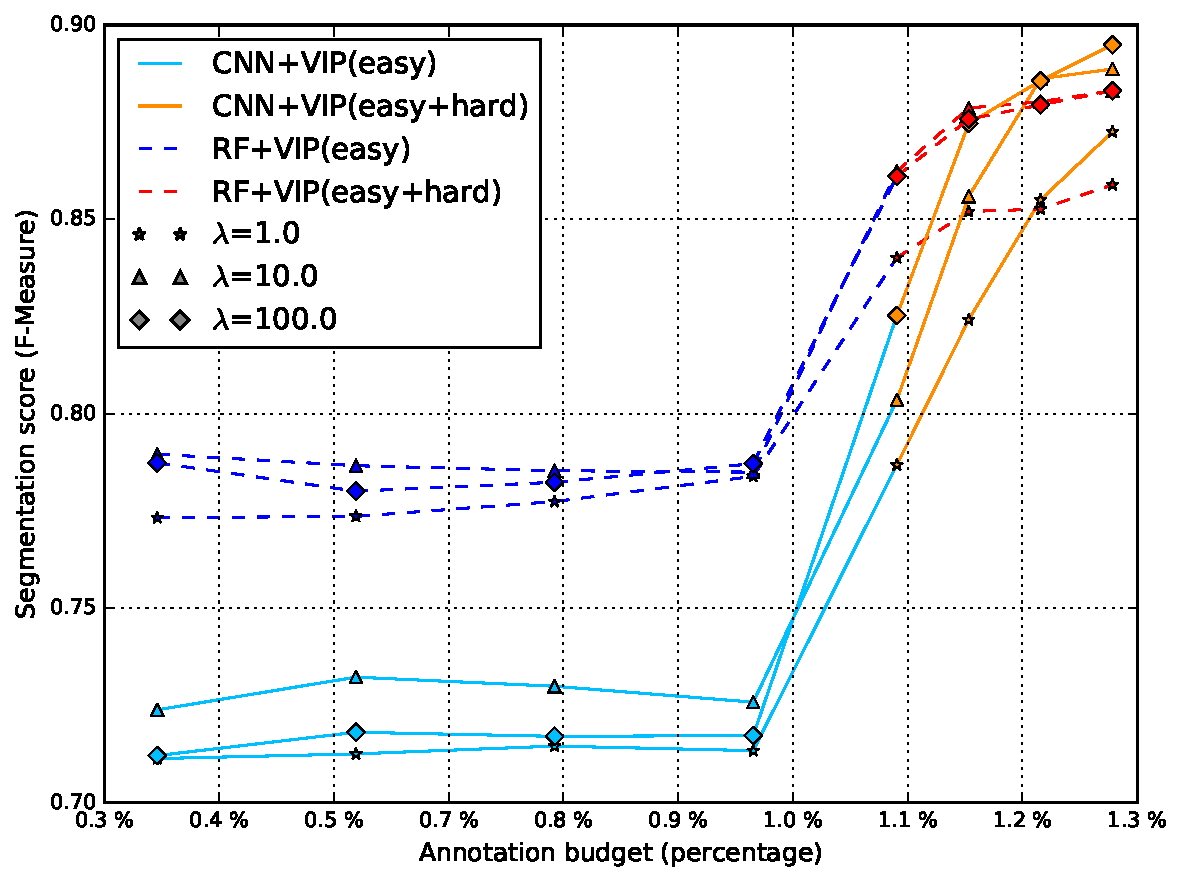
\includegraphics[width=0.8\linewidth]{figures/cnn_vs_rf_vip.pdf} 
\caption{(a) CNN with VIP (different $\lambda$)\, (b) CNN vs RF with VIP}
\end{figure}